

%%%%%%%%%%%%%%%%%%%%%%%%%%%%%%%%%%%%%%
% Chapter title 
\chapter{\textbf{Exercise} Guide}

\section{Chapter 1} 

\noindent \textbf{Exercise~\ref{ex:primelist}} \\
2	3	5	7	11	13	17	19	23	29
31	37	41	43	47	53	59	61	67	71
73	79	83	89	97	101	103	107	109	113
127	131	137	139	149	151	157	163	167	173
179	181	191	193	197	199	211	223	227	229
233	239	241	251	257	263	269	271	277	281 ... 

\noindent \textbf{Exercise~\ref{ex:primepatterns}} \\ 
Code to generate grid: \url{https://editor.p5js.org/jedediyah/sketches/tkIOKHCnb} 
\begin{center}
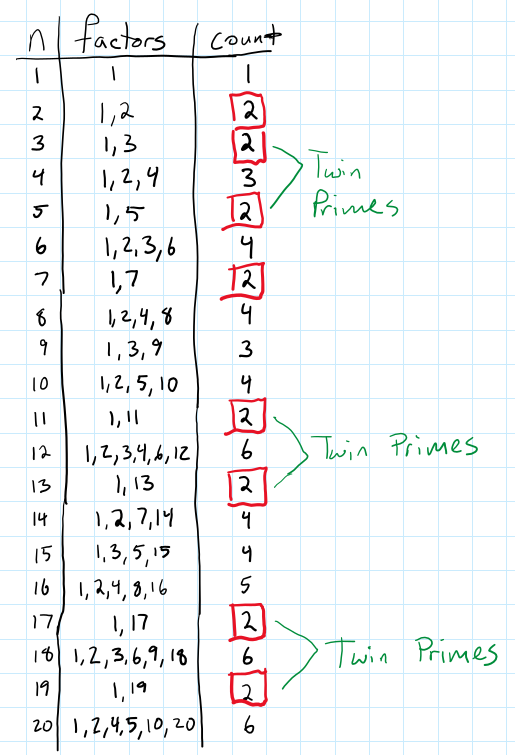
\includegraphics[width=0.3\textwidth]{img/factor-table.png}
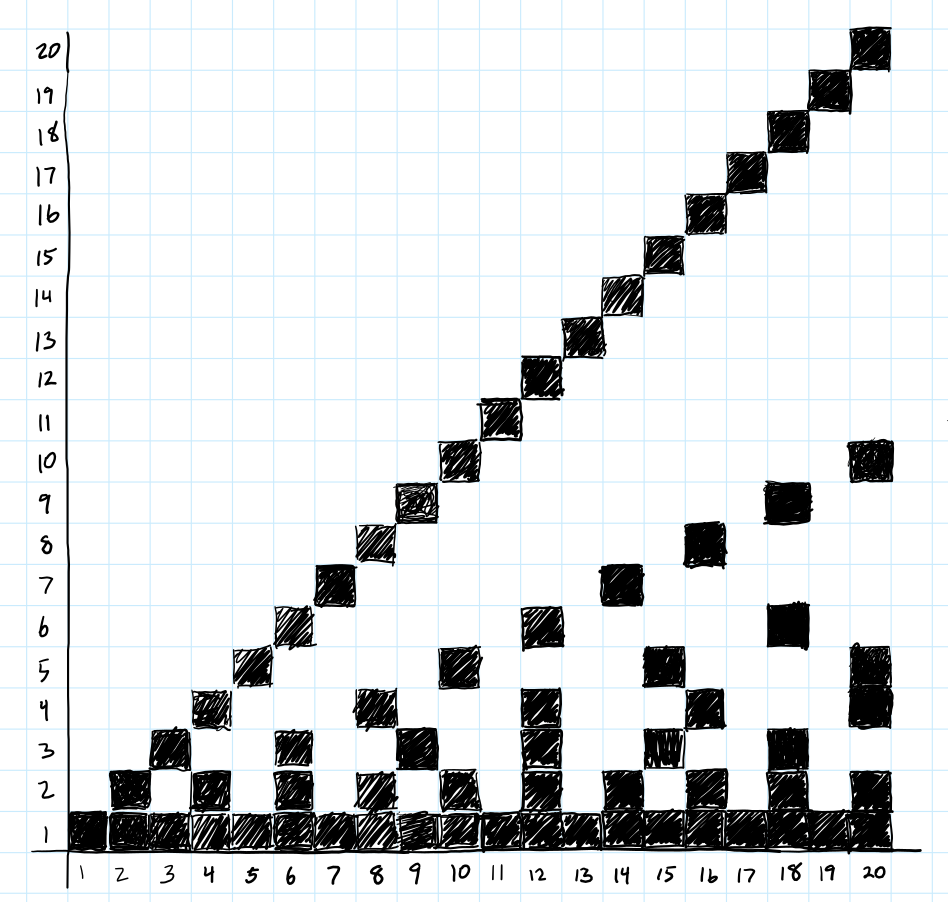
\includegraphics[width=0.5\textwidth]{img/factor-grid.png}
\end{center}

\noindent \textbf{Exercise~\ref{ex:gcdgrid}} \\
Code to generate grid: \url{https://editor.p5js.org/jedediyah/sketches/7z_OoIwHb}

\noindent \textbf{Exercise~\ref{ex:basicexponents}} \\
\(2^{5} = 32\)
